\documentclass[
    iai, % Saisir le nom de l'institut rattaché
    eai, % Saisir le nom de l'orientation
    %confidential, % Décommentez si le travail est confidentiel
]{heig-tb}

\usepackage[nooldvoltagedirection,european,americaninductors]{circuitikz}

\signature{signature.svg}

\makenomenclature
\makenoidxglossaries
\makeindex

\addbibresource{bibliography.bib}

\input{nomenclature}
\input{acronyms}
\input{glossary}
% Auteur du document (étudiant-e) en projet de Bachelor
\author{Tristan Lieberherr}

% Activer l'option pour l'accord du féminin dans le texte
\genre{male}

% Titre de votre travail de Bachelor
\title{Gestion centralisée des demandes de travaux pour le FabLab HEIG-VD}

% Le sous titre est optionnel
\subtitle{Travail de Bachelor}

% Nom du professeur responsable
\teacher {Prof. Y. Chevallier (HEIG-VD)}

% Mettre à jour avec la date de rendu du travail
\date{\today}

% Numéro de TB
\thesis{7212}



\surroundwithmdframed{minted}
\graphicspath{{assets/figures/}}

%% Début du document
\begin{document}
\selectlanguage{french}
\maketitle
\frontmatter
\clearemptydoublepage

%% Requis par les dispositions générales des travaux de Bachelor
\preamble
\authentification

%% Résumé / Version abbrégée
\begin{abstract}
  % Francais
Le but de ce travail de Bachelor est de mettre en place une plateforme web dédiée à la demande de travaux pour le FabLab.
Actuellement, la procédure est mal définie : les échanges se font manuellement par email et il n'y a pas de suivi des commandes traçable, ce qui peut impliquer des confusions, des retards de fabrication, etc.

Avec cette nouvelle plateforme, la procédure sera claire et automatisée.
Les techniciens et les clients pourront communiquer entre eux en temps réel et auront la possibilité d'avoir une vue de l'avancement du projet.
Un système de notification personnalisable sera disponible pour informer rapidement les utilisateurs concernant l'avancement de leurs demandes.
De plus, le système sera réactif : il sera accessible et ergonomique autant sur un PC que sur un smartphone.

L'interface utilisera l'authentification via Switch AAI, le même service qui est utilisé pour se connecter à son compte GAPS ou Cyberlearn, ce qui signifie que tous les étudiants y auront directement accès, sans avoir à se créer un compte.

\asterism

% English
The goal of this Bachelor's thesis is to create a web platform for submitting job requests to the FabLab.
Currently, the procedure is not well defined : communication is manually done by email and there is no way to monitor the job's progress, wich may cause confusions, production delays, etc.

With this new platform, the procedure will be clear and automated.
Both technicians and clients will be able to communicate in real time and have access to an overview of the job's progress.
A customizable notification system will be available to quickly inform the users about their job's progress.
Furthermore, the system will be reactive : it will be available and adaptive for both PC and smartphone screens.

The interface will use Switch AAI's authentication, the same service that is used to connect to GAPS or Cyberlearn, wich means that all students will have direct access, without the need to create an account.
\end{abstract}

%% Sommaire et tables
\clearemptydoublepage
{
  \tableofcontents
  \let\cleardoublepage\clearpage
  \listoffigures
  \let\cleardoublepage\clearpage
  \listoftables
  \let\cleardoublepage\clearpage
  \listoflistings
}

\printnomenclature
\clearemptydoublepage
\pagenumbering{arabic}

\usemintedstyle{xcode}

%% Contenu
\mainmatter
\chapter{Introduction}
\section{Contexte}
En l'état actuel, il n'y a pas de système automatisé pour déposer des demandes de travaux au FabLab. Il faut s'adresser à un technicien et discuter avec pour pouvoir lui soumettre son projet, et attendre qu'il ait fini avant d'aller récupérer le résultat. Pendant le temps où le technicien est à l'œuvre, le client n'a aucune idée de l'état d'avancement de sa demande. En cas de souci, le technicien doit recontacter le client, lui demander des clarifications ou des fichiers, avant de pouvoir continuer.

D'après la description de la procédure actuelle, il est possible de mettre en évidence les défauts :

\begin{enumerate}
  \item Aucun suivi des travaux pour le client
  \item Echanges éparpillés : email, vocal
  \item Risque de désorganisation
  \item Manque de clarté quant à la procédure
\end{enumerate}

\section{Cas d'utilisation}
Pour répondre aux problèmes mis en évidence, j'ai imaginé la nouvelle procédure de demandes de travaux. Dans cette procédure, il y a deux acteurs :

\begin{itemize}
  \item le client : personne qui dépose la demande
  \item le technicien : personne qui s'occupe de réaliser le travail
\end{itemize}

Cas de figure :

Le client veut réaliser une pièce fraisée pour son projet multidisciplinaire. Il se connecte sur l'interface web via le login Switch AAI, comme il en a l'habitude avec les autres services proposés par l'école. Arrivé sur la page, il peut consulter la liste des travaux réalisables, avant de remplir le formulaire. Il indique le type de travail parmi ceux disponibles, y dépose éventuellement les fichiers nécessaires et envoie la demande. Il peut voir que sa demande figure désormais dans sa liste de demandes.

Du côté du technicien, il a accès à la liste de tous les travaux déposés. Quand il voit la nouvelle demande, il se l'attribue et peut désormais voir toutes les informations du travail : type, fichiers, commentaire et messages. Lorsqu'il se met au travail, il fait changer l'état de la demande, pour que le client puisse consulter l'avancement.
Malheureusement, il manque un fichier crucial pour la réalisation et il se retrouve bloqué. Il change l'état de la demande, et envoie un message instantané au client, lui demandant d'ajouter le fichier manquant.

Quand le client est notifié par mail de ce changement d'état, il se connecte et voit qu'il a reçu un nouveau message lui demandant d'ajouter le fichier. C'est donc ce qu'il fait : il ajoute le fichier et remercie le technicien de l'avoir prévenu.

Le technicien, notifié par l'ajout du fichier, télécharge ce dernier et peut se remettre au travail. Lorsque le travail est terminé, il l'indique pour que le client puisse venir chercher la pièce.

Le client, une fois la pièce récupérée et le technicien remercié, évalue la qualité du travail avant de disposer de la demande désormais accomplie.

\figi{BPMN.xml}{14cm}{Diagramme BPMN du cas d'utilisation}

Bien sûr, les échanges seront disponibles en toutes circonstances, dès lors que le travail a été assigné à un technicien. Les acteurs pourront en tout temps s'échanges des messages instantanés et des fichiers.

\newpage
\section{Cahier des charges}
Le cahier des charges à été établi dès le début du projet et n'a pas eu besoin d'être mis à jour par la suite.
Dans ce cahier des charges, je me suis engagé à réaliser les tâches suivantes :

\begin{enumerate}
  \item Réaliser une interface Web pour la demande de travaux, qui comporte au moins les fonctionnalités suivantes :
        \begin{itemize}
          \item Liste des prestations offertes.
          \item Faire une demande de travail pour une des prestations offertes.
          \item Suivi en temps réel de l'état d'avancement de la demande.
          \item Échange de fichiers et de messages avec le technicien.
          \item Personnaliser les notifications par email.
          \item Les techniciens ont accès aux demandes de travaux déposées par les clients.
          \item Les techniciens peuvent faire évoluer le status de la demande.
        \end{itemize}
  \item Assurer une interface responsive et réactive (depuis smartphone).
  \item Architecturer la base de données.
  \item Coder le backend : ORM, gestion des demandes, notifications.
  \item Déployer l'interface sur une VM de l'école.
  \item Réaliser les tests de fonctionnement.
\end{enumerate}
\bigskip
Ce cahier des charges garantit que le système final de ce projet sera opérationnel.

\newpage
\section{Analyse des besoins et fonctions}
En fonction du cahier des charges et du cas d'utilisation, j'ai pu relever les besoins des utilisateurs.
Je les ai regroupés en deux tableaux, pour les clients et les techniciens.

\begin{table}[h]
  \begin{center}
    \caption{Besoins des clients}
    \begin{tabularx}{\textwidth}{cXc}
      No.  & Besoin                                                                                                         \\ \toprule
      N1.1 & Être capable de déposer des demandes de travaux                                                                \\ \midrule
      N1.2 & Être capable de consulter les demandes déposées et leur état d'avancement, fichiers joints et messages envoyés \\ \midrule
      N1.3 & Besoin d'être averti en étant hors-ligne d'évènements liés aux demandes                                        \\ \midrule
      N1.4 & Nécessité de pouvoir communiquer efficacement avec le technicien, d'échanger des messages et des fichiers      \\ \midrule
      N1.5 & Pouvoir accéder et interagir avec l'interface depuis un PC ou un Smartphone                                    \\ \midrule
      N1.6 & Besoin de récupérer et d'évaluer le travail accompli                                                           \\ \midrule
    \end{tabularx}
  \end{center}
\end{table}

\begin{table}[h]
  \begin{center}
    \caption{Besoins des techniciens}
    \begin{tabularx}{\textwidth}{cXc}
      No.  & Besoin                                                                                                          \\ \toprule
      N2.1 & Avoir la possibilité de consulter les demandes non assignées et de se les assigner                              \\ \midrule
      N2.2 & Être capable de consulter les demandes assignées et leur état d'avancement, fichiers joints et messages envoyés \\ \midrule
      N2.3 & Être capable de mettre à jour l'état d'avancement des commandes assignées                                       \\ \midrule
      N2.4 & Besoin d'être averti en étant hors-ligne d'évènements liés aux demandes                                         \\ \midrule
      N2.5 & Nécessité de pouvoir communiquer efficacement avec le client, d'échanger des messages et des fichiers           \\ \midrule
      N2.6 & Pouvoir accéder et interagir avec l'interface depuis un PC ou un Smartphone                                     \\ \midrule
    \end{tabularx}
  \end{center}
\end{table}

\newpage
Afin de répondre à ces besoins identifiés, j'ai pu établir le tableau des fonctions, qui liste les fonctionnalités auxquelles les utilisateurs auront accès.
Ces fonctions sont celles de base, ce qui signifie qu'il pourrait y en avoir plus dans le système final.

\begin{table}[h]
  \begin{center}
    \caption{Fonctions du système}
    \begin{tabularx}{\textwidth}[t]{p{0.5cm}Xp{1cm}}
      No. & Fonction                                                                                                                                                                                   & Besoin No.         \\ \toprule
      F1  & Créer une nouvelle demande de travaux via un formulaire adaptatif en fonction du type de travail, avec possibilité de joindre des fichiers et un commentaire à l'intention des techniciens & N1.1               \\ \midrule
      F2  & Visualiser une liste des travaux déposés ou assignés, contenant pour chaque demande toutes les informations associées                                                                      & N1.2 \newline N2.2 \\ \midrule
      F3  & Visualiser une liste de tous les travaux non assignés, contenant pour chaque demande les informations du formulaire                                                                        & N2.1               \\ \midrule
      F4  & Possibilité de s'assigner des demandes non assignées                                                                                                                                       & N2.1               \\ \midrule
      F5  & Echanger des messages instantanés depuis un salon de discussion lié à une demande                                                                                                          & N1.4 \newline N2.5 \\ \midrule
      F6  & Ajouter des fichiers à une demande                                                                                                                                                         & N1.4 \newline N2.5 \\ \midrule
      F7  & Possibilité de personnaliser les notifications par mail en fonction des évènements liés à une demande                                                                                      & N1.3 \newline N2.4 \\ \midrule
      F8  & Modifier l'état des demandes                                                                                                                                                               & N2.3               \\ \midrule
      F9  & Adaptation automatique de l'interface graphique au type et à la taille de l'écran de l'appareil utilisé                                                                                    & N1.5 \newline N2.6 \\ \midrule
      F10 & Suppression d'une demande terminée                                                                                                                                                         & N1.6               \\ \midrule
      F11 & Evaluation du travail accompli                                                                                                                                                             & N1.6               \\ \midrule
    \end{tabularx}
  \end{center}
\end{table}

\newpage
\section{Choix technologiques}
Le monde du développement web est un univers totalement nouveau pour moi.
Au cours de ma formation, j'ai acquis des compétences très basiques en HTML, PHP et JavaScript.
Je n'ai par conséquent jamais utilisé de framework auparavant.

Après avoir exploré le net et consulté mon mentor, j'ai découvert qu'il existait une multitude de frameworks.
J'ai ensuite sommairement rempli un tableau qui regroupe certains des frameworks populaires afin d'établir un comparatif, pour mettre en évidence les avantages et les inconvénients de chacun.
Étant donné la prédisposition pour le framework backend Laravel, comme expliqué plus loin, j'ai limité le nombre de frameworks backend dans le tableau.

Pourquoi avoir choisi les plus populaires ? En général, si un outil est populaire, il sera facile de trouver des réponses et des solutions sur internet.
En vérifiant sur StackOverflow, j'ai trouvé des graphiques qui appuient mon propos.

\begin{table}[h]
  \begin{center}
    \caption{Comparaison des bases de données \label{specification}}
    \begin{tabularx}{\textwidth}[t]{m{1cm}Xp{4cm}p{4cm}}
      No.                               & Technologie     & Avantages & Inconvénients \\ \toprule
      1                                 & MySQL           & 
      \textbf{+} DB relationnelle \newline
      \textbf{+} Très populaire
                                        & 
      \textbf{--} Convient mal pour stocker énormément de données                     \\ \midrule
      2                                 & MongoDB         & 
      \textbf{+} Performant             & 
      \textbf{--} Non relationnelle                                                   \\ \midrule
      3                                 & PostgreSQL      & 
      \textbf{+} Riche en fonctionnalités \newline
      \textbf{+} DB relationnelle/objet & 
      \textbf{--} Plus complexe que MySQL                                             \\ \midrule
      4                                 & Oracle Database & 
      \textbf{+} DB relationnelle       & 
      \textbf{--} Payant                                                              \\ \midrule
    \end{tabularx}
  \end{center}
\end{table}

\begin{table}[h]
  \begin{center}
    \caption{Comparaison des frameworks frontend \label{specification}}
    \begin{tabularx}{\textwidth}[t]{m{1cm}Xp{4cm}p{4cm}}
      No. & Technologie & Avantages & Inconvénients \\ \toprule
      1   & Angular     & 
      \textbf{+} Très complet
          & 
      \textbf{--} Complexe
      \\ \midrule
      2   & React       & 
      \textbf{+} Simple
          & 
      \textbf{--} JavaScript XML (JSX)
      \\ \midrule
      3   & Vue         & 
      \textbf{+} Simple \newline
      \textbf{+} Le site PIAF est en Vue
          & 
      \textbf{--} Trop flexible
      \\ \midrule
    \end{tabularx}
  \end{center}
\end{table}

\begin{table}[h]
  \begin{center}
    \caption{Comparaison des frameworks backend \label{specification}}
    \begin{tabularx}{\textwidth}[t]{m{1cm}Xp{4cm}p{4cm}}
      No. & Technologie & Avantages & Inconvénients \\ \toprule
      1   & Laravel     & 
      \textbf{+} Simple \newline
      \textbf{+} Professeur expérimenté
          & 
      \textbf{--} Convient moins bien aux gros projets
      \\ \midrule
      2   & Django      & 
      \textbf{+} Développement rapide
          & 
      \textbf{--} Python
      \\ \midrule
      3   & Express     & 
      \textbf{+} JavaScript
          & 
      \textbf{--} Nature asynchrone compliquée
      \\ \midrule
      4   & Rails       & 
      \textbf{+} Simple
          & 
      \textbf{--} Ruby
      \\ \midrule
    \end{tabularx}
  \end{center}
\end{table}

J'ai évidemment dû me fier à l'avis des auteurs, car ne connaisant rien, il m'a parfois été difficile de vraiment comprendre les différences entre les outils.
Néanmoins, j'ai pu me faire une idée quant à ce qui existe dans le milieu.

%% https://www.trustradius.com/products/laravel-php-framework/reviews?qs=pros-and-cons

\figi{stackoverflow_trends_frontend.svg}{14cm}{StackOverflow, questions par mois, frontend}
%% https://insights.stackoverflow.com/trends?tags=reactjs%2Cvue.js%2Cangular%2Cangularjs


\figi{stackoverflow_trends_backend.svg}{14cm}{StackOverflow, questions par mois, backend}
%% https://insights.stackoverflow.com/trends?tags=laravel%2Cdjango%2Cexpress%2Cruby-on-rails

\figi{stackoverflow_trends_DB.svg}{14cm}{StackOverflow, questions par mois, database}
%% https://insights.stackoverflow.com/trends?tags=mysql%2Cmongodb%2Cpostgresql%2Coracle

%% https://trends.google.fr/trends/explore?date=today%205-y&q=%2Fg%2F11c0vmgx5d,%2Fg%2F11c6w0ddw9,%2Fm%2F012l1vxv
%% https://trends.google.fr/trends/explore?date=today%205-y&q=Laravel,%2Fm%2F06y_qx,%2Fm%2F0_v2szx,%2Fm%2F0505cl
%% https://trends.google.fr/trends/explore?date=today%205-y&q=%2Fm%2F04y3k,%2Fm%2F05ynw,%2Fm%2F05z_r2n,%2Fm%2F01vw9z

Au final, ce sont les frameworks Vue et Laravel que j'ai choisi, ainsi que la base de données MySQL.

Pourquoi Vue ? Car la raison principale est que l'institut IAI possède un site template qui utilise Vue, auquel j'ai pu avoir accès.
Toute la structure du site était déjà faite, ce qui procure un gain de temps énorme.
C'est aussi pour ça que je n'ai inclu que React et Angular dans mon comparatif : avec Vue, ils forment ensemble les principaux frameworks frontend.
Vue est aussi un framework très simple pour les débutants, et qui gagne en popularité.
Il est apparement très bien documenté et il existe des bibliothèques gratuites de composants.

Pourquoi Laravel ? Car c'est un framework très simple pour les débutants comme moi, et que le professeur Chevallier sait s'en servir.
En cas de problèmes, il saura m'aider et m'orienter, ce qui selon moi justifie pleinement son utilisation.

Pourquoi MySQL ? Car c'est ce qui semble être LA base de données par défaut. Elle est gratuite, populaire, et à défaut d'avoir besoin de spécifications particulières en terme de performances, convient très bien à n'importe quel projet.
Il fallait aussi que ce soit une base relationnelle, c'est à dire avec des tables de modèles définis.


\section{Spécifications}
\section{Matériel nécessaire}
\chapter{Vue d'ensemble}

Avant de parler en détail des aspects techniques, ce chapitre a pour but de dresser une vue d'ensemble des composants du système, afin de se familiariser avec son fonctionnement.

\section{Pages web}

La structure d'un site est assez simple : c'est un ensemble de pages consultables à la demande. Chaque page possède du code HTML, responsable de la mise en forme du contenu, et du code JavaScript, qui permet d'exécuter des actions, par example quand on clique sur un bouton.
Quand vous naviguez sur un site, vous avez accès à une arborescence de pages, chacunes identifiées par une addresse, une route : il s'agit de l'URL, le texte visible en haut du navigateur.

Dans le cadre de ce chapitre, nous avons affaire à deux principales entités distinctes :
\begin{itemize}
  \item Le serveur : la machine qui s'occupe de servir les pages et les données aux clients
  \item Le client : la machine qui avec son navigateur essaie d'accéder au site
\end{itemize}
\bigskip
L'utilisateur est la personne physique qui veut accéder au site. Son appareil (PC, Smartphone) est le client.

Pour accéder à une page, le navigateur doit envoyer une requête HTTP au serveur. Le serveur lui répond en lui retournant la page à afficher.
C'est pareil pour toutes les pages : le navigateur doit à chaque fois envoyer une requête et attendre la réponse avant de l'afficher.

\figi{figure1.xml}{12cm}{Site traditionnel}

Cette méthode, bien que parfaitement fonctionnelle, possède toutefois des inconvénients :
\begin{itemize}
  \item Il faut envoyer et attendre la réponse de la requête pour chaque page, ce qui prend du temps
  \item Il n'a a pas de mise à jour automatique du contenu : il faut actualiser la page, donc renvoyer une requête
  \item Le trafic réseau peut être élevé en raison des nombreuses requêtes
\end{itemize}
\bigskip
Heureusement, au fil des années, le monde du web s'est fortement développé et il existe une nouvelle façon de faire.
Cette méthode consiste non plus à envoyer les pages à la demande, mais à envoyer toutes les pages à la fois, et à laisser le navigateur s'occuper de leur accès.

C'est à dire qu'au lieu de demander une nouvelle page à chaque fois, le navigateur, qui la possède déjà, va l'afficher directement sans envoyer de requête au serveur.
Ce fonctionnement implique qu'il n'y a que très peu de temps d'attente pour l'affichage de la nouvelle page, ce qui améliore considérablement le confort de l'utilisateur.

\figi{figure2.xml}{12cm}{Site SPA}

Désormais, un site n'est plus juste un assortiment de pages inertes et figées, c'est devenu une sorte d'entité "vivante", à la façon d'une application.
On appelle ce type de site une "SPA" pour \emph{Single Page Application}.
Cela dit, il peut encore y avoir des requêtes, sauf que cette fois, il ne s'agit plus de demander une page entière, mais seulement d'accéder à des ressources.

Le volume de données est considérablement réduit puisque tout le code HTML est déjà présent : il s'agit de rapatrier uniquement les données à afficher.

De plus, avec l'apparition de ces sites "intelligents", une nouvelle technologie très intéressante est apparue : celle des websockets.
Grâce aux websockets, les serveurs ont désormais la possibilité de spontanément contacter les clients pour leur envoyer des données.

En effet, sans cette technologie, les serveurs ne peuvent que reçevoir des requêtes et non pas les envoyer.

\section{Base de données et backend}

Le terme de "backend" désigne la partie du site qui s'occupe de la gestion des données, de l'authentification des utilisateurs et de l'envoi de la SPA.
Quand un client s'addresse au backend, ce dernier va effectuer des actions, par exemple pour stocker ou retourner des ressources, envoyer des mails ou encore envoyer des notifications push aux clients.

Le backend est très souvent couplé à une base de données qu'il utilise pour stocker les données du système, par example les données concernant les utilisateurs.
La base de données est un système de stockage organisé de ressources, qui permet d'insérer, d'éditer, de retirer et de supprimer les ressources qu'elle contient.
Dans le cas d'une base de données relationnelle, le stockage se fait à la manière d'un tableur : chaque ligne représente une entrée, et chaque entrée possède des attributs rangés en colonnes.

Les clients communiquent avec le backend via une API, une interface qui associe à chaque route, chaque addresse, à un type de réponse.
L'API décrit le format des données échangées, entre le code PHP côté backend et JavaScript côté frontend.

\figi{figure3.xml}{14cm}{Echanges de données entre le client et le backend}

\section{Interface utilisateur et frontend}

Le terme de "frontend" désigne la SPA, l'application qui s'occupe d'afficher les données et d'interagir avec l'utilisateur et le backend.
C'est au travers de cette SPA que l'utilisateur va accéder aux fonctionnalités.

L'avantage est que les données seront affichées en temps réel, ce qui enlève la nécessité de rafraichir la page pour s'assurer que le contenu présenté soit à jour.

C'est d'ici que se font les requêtes HTTP pour l'accès aux ressources.

\section{Aperçu d'une page Vue}
Vue est un framework permettant de développer une SPA et qui utilise principalement du JavaScript et du HTML.
L'organisation de l'interface se fait en composants, qui sont des éléments graphiques programmables.
Je trouve d'ailleurs qu'il y a une ressemblance entre ces composants et ceux utilisés en C\# WPF.

Un composant Vue est structuré de la manière suivante :
\begin{enumerate}
  \item template : c'est la partie en HTML qui décrit l'affichage du composant
  \item script : c'est ici que tout le code JavaScript est situé
  \item style : contient les classes CSS utilisées dans le template
\end{enumerate}
\bigskip
Ces composants peuvent être utilisés dans d'autres composants, et peuvent être associés à une page.
Dans Vue, une page est définie par une route (URL) qui est associée à un fichier qui contient un composant.
Lorsque la page est appelée, le routeur Vue s'occupe d'afficher le bon composant.

Pour communiquer entre les composants, il y a deux façons de faire :
\begin{itemize}
  \item Le parent transmet des données à l'enfant par propriétés
  \item L'enfant transmet des données au parent par évènement
\end{itemize}
\bigskip
\newpage

Pour ce faire, il existe des directives spéciales.
La plus utilisée est la directive "v-on", abrégée avec le symbole ":", qui permet de passer une variable à une propriété.
Pour utiliser les évènements, on peut utiliser le symbole "@" devant le nom de l'évènement pour lui associer une fonction.
Prenons un example :
\begin{minted}{html}
  <composant :name="userName" surname="Tristan" @click="componentClicked">
    ...
  </composant>
\end{minted}
Dans cet exemple, la variable "userName" est passée à la propriété "name", tandis que la chaine de caractères "Tristan" est passée à "surname".
Lorsque la composant émet l'évènement "click", c'est la méthode "componentClicked" qui va être appelée.

Dans le script d'un composant, on a accès à plusiers fonctionnalités :
\begin{itemize}
  \item components : permet d'importer d'autres composants
  \item data : contient les variables du composant
  \item methods : déclaration des méthodes
  \item computed : ce sont des sortes de méthodes sans paramètres qui retournent des variables modifiées
  \item watch : callbacks appellés quand une variable change
\end{itemize}
\bigskip
Il existe encore des méthodes qui sont appellées automatiquement durant le cycle de vie du composant, comme par exemple mounted(), destroyed(), ...
\newpage
\inputminted[breaklines]{html}{assets/code/component_example.vue}

\chapter{Architecture de la base de données}
\section{Modèles}
L'élaboration des modèles est une partie essentielle du développement car il s'agit de déterminer quelles informations il faut stocker pour pouvoir faire fonctionner le système.
Ces modèles ont évolué avec le temps, car il a fallu les adapter au fur et à mesure que des fonctionnalités ont été ajoutées.
\figi{db_schema.svg}{14cm}{Schéma de la base de données}

\chapter{Conception du frontend}
%% https://themeforest.net/item/piaf-vuejs-admin-dashboard/23160320
Afin de partir depuis une bonne base, Mr. Chevallier a pu partager avec moi un site préfait, acheté par l'institut IAI.
J'ai pu forker le repo sur GitHub, et à partir de là, j'ai pu commencer à réaliser le frontend.
Je n'ai donc pas eu à créer un projet Vue à partir de zéro, et les pages déjà présentes m'ont servi d'exemple lors de mon apprentissage du framework.

\section{Cycle de vie d'une demande}
Dés lors de sa création, une demande va passer par plusieurs étapes tout au long de son cycle de vie : ces étapes sont caractérisées par son statut.
Le statut est l'indication de l'état d'avancement de la demande, et c'est donc cette propriété que le technicien peut faire évoluer.

Pour qu'un technicien puisse faire avancer l'état de la demande, il doit d'abord se l'assigner.
Une demande non assignée ne peut pas encore être modifiée : elle ne peut être que consultée par les techniciens.
Une fois assignée, la demande n'est plus visible des autres techniciens et n'est accessible que par le client demandeur et par le technicien responsable.

Une demande possède trois éléments importants : des messages, des fichiers et une timeline.
La timeline peut contenir les évènements suivants :
\begin{itemize}
  \item Changement de statut.
  \item Ajout d'un fichier.
\end{itemize}
\bigskip

L'assignation débloque la possibilité d'envoyer de messages instantanés et d'ajouter des fichiers.
Avant ça, ces fonctionnalités sont bloquées : une demande peut toutefois déjà contenir les fichiers ajoutés depuis le formulaire.
Les évènements de la timeline sont générés automatiquement, donc cette fonction n'est jamais accessible par les utilisateurs.

Au tout début, le client doit remplir le formulaire de nouvelle demande et la soumettre.
Il n'y a que les clients qui peuvent faire une nouvelle demande : les techniciens ne peuvent que les assigner.
La nouvelle demande commence au premier stade, avec le status "NEW".
\newpage

Le diagramme ci-dessous représente les différents statuts et stades que la demande va atteindre, dans l'ordre chronologique.

\figi{lifecycle.xml}{12cm}{Cycle de vie d'une demande}

\begin{enumerate}
  \item[Stade 1.] La demande est toute nouvelle. Elle n'a pas encore été assignée à un technicien, part conséquent il n'est pas encore possible d'échanger des messages ou d'ajouter des fichiers. Ce statut initial est automatique.
  \item[Stade 2.] La demande à été assignée à un technicien, donc il y a désormais une prise en charge du travail. Il peut maintenant y avoir des échanges de messages et des fichiers peuvent êtres ajoutés. Ce statut est automatiquement mis à jour quand la demande est assignée.
  \item[Stade 3.] La demande est soit en cours de production, soit en arrêt. Ces deux statuts peuvent êtres interchangés manuellement par le technicien. Le mode "ON HOLD" indique au client que le travail à dû être mis en attente à cause d'un problème. C'est aux deux acteurs de discuter entre eux pour le régler.
  \item[Stade 4.] Le travail est terminé. Ce statut est atteignable manuellement. Le client est en mesure de venir chercher le travail accompli, et peut désormais supprimer la demande, après avoir évalué la qualité du travail.
\end{enumerate}
\bigskip
Certains de ces statuts sont attribués automatiquement, c'est le cas de "NEW" et de "ASSIGNED".
Tous les autres sont modifiables par le technicien.

Ces noms de statuts sont en anglais, bien que le reste de l'interface soit en français.
Cette particularité est voulue, car comme il s'agit d'un nom de code, j'ai trouvé élégant d'utiliser de l'anglais.

\newpage
\section{Premier croquis de l'interface}
Avant de commencer à coder, j'ai réalisé quelques croquis pour définir grossièrement à quoi allait ressembler l'interface du site.
Au final, l'apparence a beaucoup été infulencée par les composants issus de bibliothèques externes (Vuetify) et par la forme du site de base.
Néanmoins, mes croquis ont servi de base pour le placement de ces composants.
Il faut noter que ces croquis ne traitent que de la version PC de l'interface : les différentes pages devront accomoder un petit écran tactile et par conséquent l'interface risque de changer en fonction.
De plus, de nouvelles pages sont apparues au fil du temps, et il n'existe pas de croquis de base pour ces dernières : c'est donc normal qu'il n'y ait pas autant de croquis que de pages ou de fenêtres.

Pour naviguer sur le site, j'ai décidé d'utiliser un overlay, c'est à dire deux barres fixes sur le haut et sur la gauche qui contiennent les liens vers les pages.
La barre de gauche peut être masquée pour bénéficier de pages qui prennent toute la largeur.

\figi{ui_overlay.xml}{10cm}{Croquis de l'overlay}

Ce style est assez standard puisqu'on le rencontre sur de nombreux sites (Cyberlearn, Vuetify, Laravel docs, ...).
C'est d'ailleurs celui qui était utilisé dans le site de base.
On y retrouve certains éléments habituels, comme la cloche de notifications ou le nom de l'utilisateur qui permet de dérouler un menu.

\newpage
Pour pouvoir modifier les paramètres de notifications par mail, j'ai imaginé une page exprès pour.
Sur cette page sont aussi affichées quelques informations de base concernant le compte de l'utilisateur, comme le nom, l'adresse mail et le nombre de demandes actives.

\figi{ui_settings.xml}{10cm}{Croquis de la page des paramètres}

Pour pouvoir déposer une demande, j'ai voulu mettre une liste des travaux disponibles avec une image et une description de chaque machine.
Si tous les acteurs peuvent voir cette liste, seuls les clients peuvent déposer une demande.
Pour ce faire, j'ai imaginé un formulaire dans lequel il faut indiquer le type de travail, la date de rendu et les fichiers nécessaires.
J'ai aussi voulu mettre un champ de texte pour que le client puisse ajouter un commentaire optionnel à l'intention des techniciens.

\figi{ui_submit_job.xml}{14cm}{Croquis de la liste des travaux disponibles et du formulaire}

\newpage
Pour consulter leurs demandes, les utilisateurs doivent pouvoir y avoir accès rapidement et idéalement avoir la possibilité de les trier.
Pour réaliser cette tâche, j'ai pensé à utiliser un tableau, avec une fonction de tri.
Ce tableau existe : il s'agit du composant "v-data-table" de la bibliothèque Vuetify.
Je n'ai donc pas eu besoin de faire de croquis pour ça.

J'ai aussi décidé de créer une fenêtre qui donne une vue d'ensemble sur la demande sélectionnée.
Cette fenêtre est le "hub" central d'une demande, puisqu'elle contient toutes les informations de la demande : statut, fichiers, timeline, messagerie, ...
Toutes ces informations au même endroit, tel était la motivation pour la réalisation de ce composant.

\figi{ui_jobinfo.xml}{10cm}{Croquis des détails d'une demande}

La fenêtre offre des fonctionnalités différentes pour les clients et les techniciens.
Par exemple, un technicien peut changer l'état de la demande, tandis que le client à la possibilité de supprimer la demande un fois qu'elle est terminée.

\newpage
\section{Interface finale}
Le résultat final à été basé sur les croquis, bien que les composants de la bibliothèque Vuetify aient fortement influencé le design.
Il y a donc eu beaucoup de nouveautés par rapport aux croquis de base, qui ne couvraient que quelques vues.

On retrouve le même overlay, avec en plus le logo central qui est un lien vers la page "Mes commandes".
Le bouton tout à gauche sert à basculer la visibilité de la barre latérale.
La cloche de droite indique le nombre de notifications es contient aussi un lien vers la page "Mes commandes".
Si on clique sur le nom à côté de la cloche, un menu permettant de se déconnecter apparait.

La première page de la liste est celle des paramètres.
Cette page ressemble beaucoup à ce qui était prévu dans le croquis.
Pour modifier les options, des boutons de type "switch" sont utilisés.
Ces boutons sont avantageux puisqu'ils indiquent directement leur état : ON ou OFF.

Par souci de confort, il est possible de d'activer ou de désactiver toutes les options d'un coup.

\begin{figure}[h!]
  \makebox[\textwidth]{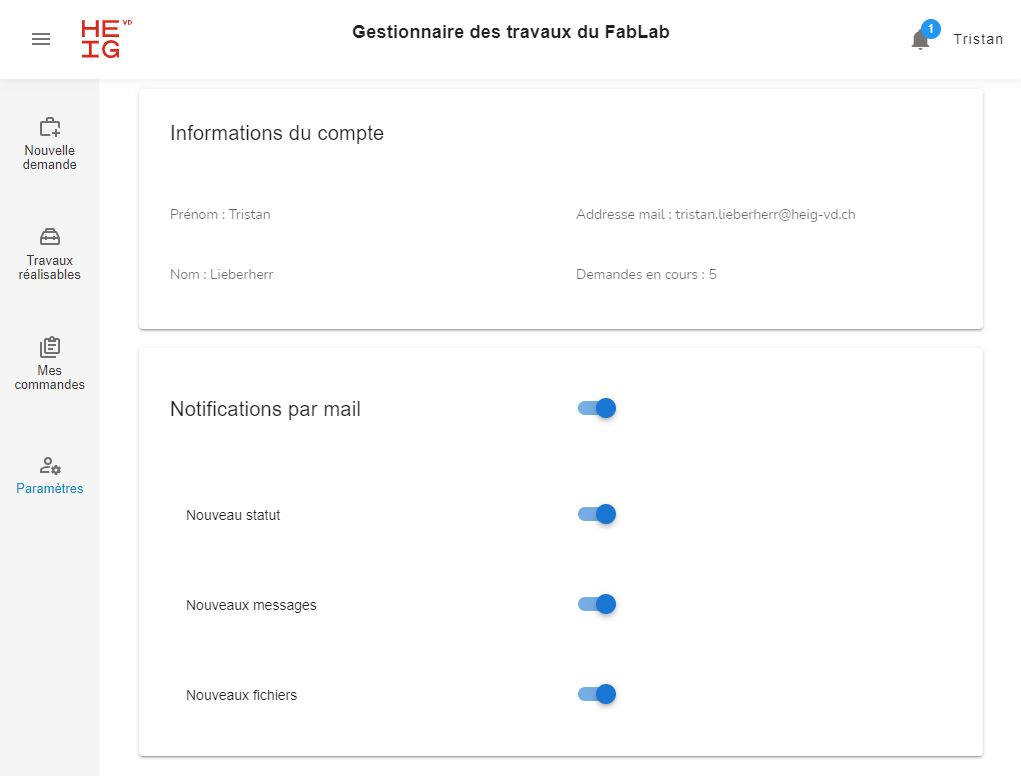
\includegraphics[width=14cm]{ui_settings_page.PNG}}
  \caption{Page des paramètres du technicien}
\end{figure}

Côté fonctionnement, ils sont synchronisés avec le serveur, donc l'état affiché correspond à l'état mémorisé.
Il n'y a pas besoin d'appliquer les modifications, puisqu'elles se font directement lors du changement d'état des boutons : une petite animation de chargement indique que les modifications sont en train d'être appliquées, ce qui indique à l'utilisateur que les changements sont biens enregistrés.

\newpage
La seconde page contient un tableau de toutes les demandes déposées ou attribuées : le client verra ses demandes déposées et le technicien verra celles qu'il s'est assigné.
Ce tableau peut être trié selon plusieurs critères, et quand on clique sur une des entrées, la fenêtre de détails s'ouvre.

\begin{figure}[h!]
  \makebox[\textwidth]{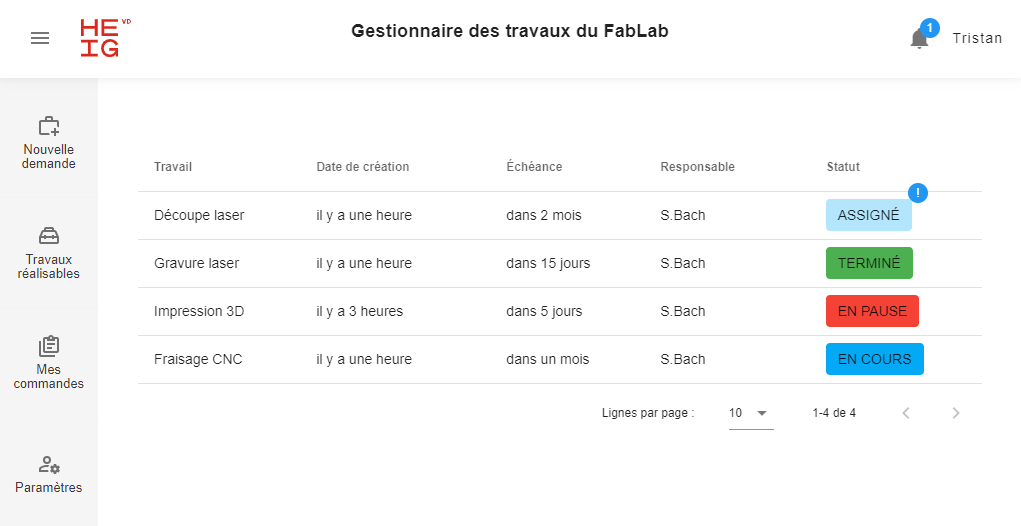
\includegraphics[width=14cm]{ui_myjobs_client.PNG}}
  \caption{Page des demandes du client}
\end{figure}

La fenêtre de détails finale est presque identique à celle qui était prévue dans le croquis.
On peut voir l'état d'avancement grâce au stepper en quatre étapes.
La chatbox permet d'afficher les messages entre les interlocuteurs.
La timeline affiche les évènements importants liés à la demande.
Pour les fichiers, un numéro de version est indiqué.
Cette indication est utile si un même fichier est modifié puis ajouté de nouveau.

\begin{figure}[h!]
  \makebox[\textwidth]{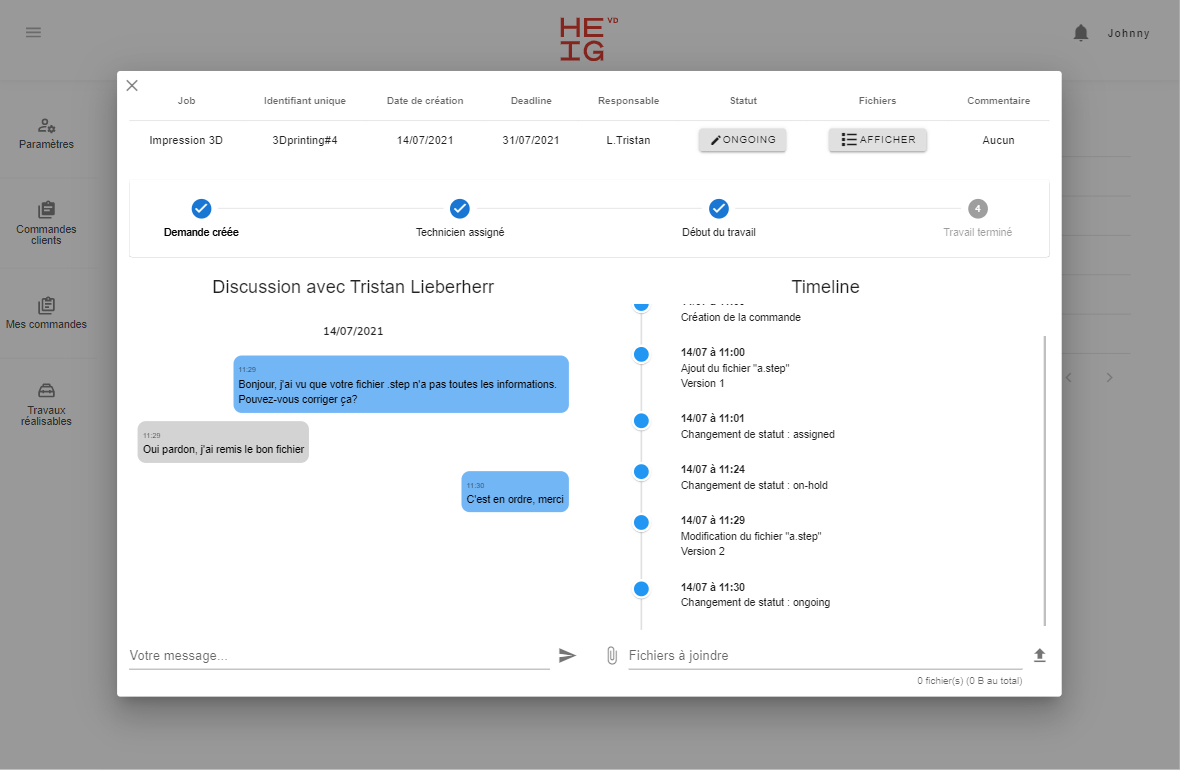
\includegraphics[width=14cm]{ui_jobinfo_tech1.PNG}}
  \caption{Détails d'une demande, côté technicien}
\end{figure}



Si l'utilisateur est un technicien, il a accès à une page supplémentaire qui contient la liste de toutes les demandes non attribuées.
Il peut voir des informations basiques concernant les demandes, comme le type de travail, la date de rendu et le commentaire.

Pour qu'un technicien puisse s'attribuer des travaux, il peut cocher la checkbox des demandes voulues, puis cliquer sur le bouton vert "Assigner".
Une fenêtre modale de confirmation apparaitra et une fois la validation faite, les demandes fraichement assignées seront ajoutées dans le tableau de la page "Mes travaux".

\begin{figure}[h!]
  \makebox[\textwidth]{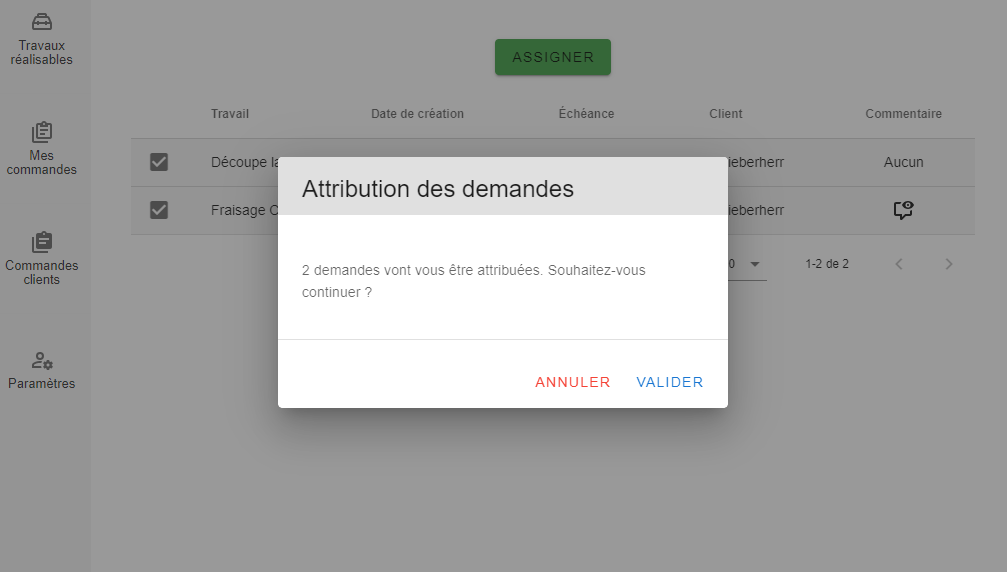
\includegraphics[width=20cm]{ui_alljobs_assign.PNG}}
  \caption{Page des travaux non-assignés}
\end{figure}

Pour voir le commentaire, s'il y en a un, il faut cliquer sur l'icône dans la colonne en question, pour faire apparaitre une petite fenêtre modale contenant le message.

\begin{figure}[h!]
  \makebox[\textwidth]{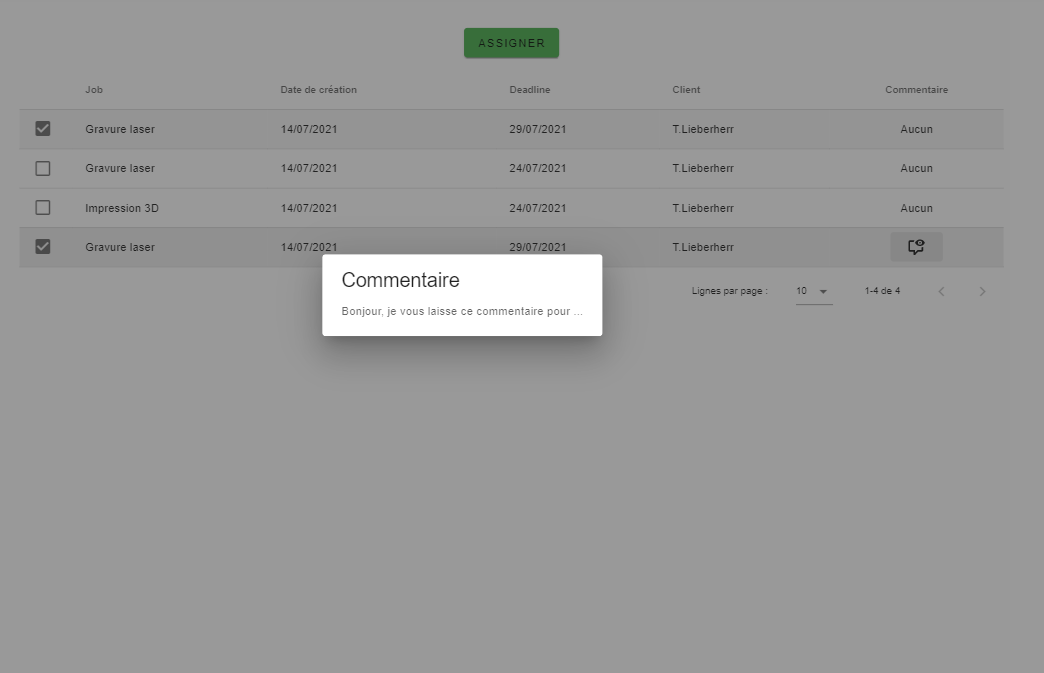
\includegraphics[width=20cm]{ui_alljobs_comment.PNG}}
  \caption{Page des travaux non-assignés, vue du commentaire}
\end{figure}

\section{Gestion des données et pattern MVC}
%% https://vuex.vuejs.org/#what-is-a-state-management-pattern
%% https://code-cartoons.com/a-cartoon-guide-to-flux-6157355ab207
La gestion des données est un aspect très important du frontend.
Pour ce faire, il existe un design pattern très populaire qui s'appelle le MVC, pour "Model View Controller".
Dans son fonctionnement, on retrouve trois parties :
\begin{enumerate}
  \item Contrôleur : c'est la partie qui gère les interactions entre l'utilisateur et les données.
  \item Modèle : c'est les données qui vont être affichées.
  \item Vue : c'est l'interface visuelle qui présente les données.
\end{enumerate}
\bigskip

Ce pattern est assez simple en terme de fonctionnement, mais il est redoutablement efficace.

\figi{MVC.xml}{14cm}{Pattern MVC}

Comme le site est de type SPA, les données nécessaires à l'affichage sont demandées au serveur par le client.
Il doit donc y avoir un endroit où les stocker : c'est là qu'intervient Vuex.
Le partage de données entre composants est un possibilité, mais Vuex offre bien trop d'avantages.

Vuex est un pattern et une librairie qui fait office de gestionnaire d'état pour les applications Vue.
Plus précisément, c'est un lieu de stockage qui peut contenir des données, et qui offre des accesseurs et des mutateurs pour interagir avec.
Ce lieu s'appelle le "store", le magasin en français.

Le premier avantage de ce système est qu'il n'y a qu'une seule instance des objets stockés dedans, une seule source de vérité accessible depuis tous les composants.
Dans Vue, les composants s'échangent des données soit par props soit par évènements.
Imaginons le cas de figure où le composant G doit accéder à une ressource qui est stockée dans le composant D.
Cette configuration peut poser de gros problèmes, car les données transitent partout et il y a des dépendances entre composants.

\newpage
\figi{vuex1.xml}{14cm}{Échange de données entre composants}

Le problème principal est que plusieurs variables risquent de posséder plusieurs états différents (des valeurs différentes) alors qu'elles devraient partager le même.
La compagnie Facebook à justement eu ce souci il y a quelques années.
Un bug s'est manifesté sous forme de notifications "fantômes", qui indiquaient de nouveaux messages alors que ce n'était en réalité pas le cas.
Les développeurs ont alors décidé de se débarasser du problème en créant Flux, un nouveau design pattern de gestion d'état, qui a inspiré Vuex par la suite.

\figi{vuex2.xml}{14cm}{Échange de données avec le store}

Avec Vuex, il n'y a pas de problème d'états différents, puisqu'il n'existe qu'un seul exemplaire de la ressource, qui est directement accessible.
Si un composant veut modifier l'état, il doit passer par un mutateur et tout changement sera propagé aux composants qui en dépendent.

\newpage
L'utilisation de mutateurs assure que les données soient modifiées de façon synchrone, contrôlée et prédictible.
Les actions servent principalement à envoyer des requêtes au serveur pour y récupérer des données.
Sur le schéma ci-dessous, on voit le cycle qui se produit lorsqu'un composant a besoin de récupérer des données depuis le serveur.
Il appelle une action (une fonction qui retourne une promesse) qui va s'occuper de la requête et de la mutation de la ressource.

\figi{vuex.xml}{14cm}{Récupération des données du serveur}

Le second avantage est que toute la partie du code qui s'occupe des requêtes HTTP est située dans les actions, ce qui fait que le code est à portée de main dans un seul fichier.
L'utilisation de Vuex a donc été très utile, surtout pour l'organisation du code et des données, et de l'application efficace du pattern MVC.
De plus, il y a la garantie qu'il n'y aura jamais de problèmes avec l'état des variables entre composants.

\chapter{Conception du backend}
\section{Présentation de Laravel}
\section{Routes API}
\section{Notifications par mail}
\section{Authentification par Switch AAI}
%% https://www.switch.ch/aai/demo/medium/
Une des fonctionnalités importante du projet est la connection au service à travers le login Switch AAI.
Le gros avantage est que les nouveaux utilisateurs n'ont pas besoin de se créer un nouveau compte.

Le déroulement et fonctionnement de l'authentification se déroule en plusieurs étapes.
Lorsque l'utilisateur veut accéder à une ressource, comme un site par exemple, il essaie d'y accéder depuis son navigateur.



\chapter{Déploiement}
\section{Serveur Apache}
\section{Serveur Websocket}
\section{Processus supervisés}




\chapter{Introduction}
L'introduction est une section requise dans un rapport technique. Introduisez votre travail, l'idée de départ et les objectifs attendus. Un lecteur qui découvrirait votre projet au travers de cette introduction devrait ainsi être capable d'en comprendre le cadre, l'idée générale et les aboutissants du projet.

\section{Contexte}
Cette section \underline{n'est pas obligatoire}, mais elle est souvent présente dans un rapport technique pour compléter l'introduction et définir le contexte du travail \cad le cadre formel dans lequel le travail est mené.

%%if
\section{Citations et bibliographie}
Citer vos sources est essentiel. Avec \texttt{biblatex} vous pouvez facilement citer des articles, des livres ou des sites internet. Toutes les citations dans le texte seront automatiquement regroupées en fin de document dans la section \guillemotleft Bibliographie\guillemotright. Par exemple, citons un article d'Einstein \cite{einstein} ou le livre de Dirac \cite{dirac}.

Parfois il peut être utile d'utiliser un gestionnaire de bibliographie. La communauté académique recommande l'outil \href{https://www.zotero.org/}{Zotero} qui permet de gérer une bibliothèque numérique d'ouvrages et de références numériques. Il permet également de générer une bibliographie compatible avec \LaTeX.

\section{Exemple d'équation}
L'une des principales forces de \LaTeX est la saisie d'équations. L'équation \ref{eq:1}, citée à titre d'exemple, représente la transformation de phase d'une lentille biconvexe. Pour rédiger une équation \LaTeX vous pouvez utiliser des outils en ligne tels que \href{https://www.latex4technics.com/}{latex4technics}.

\begin{equation} \label{eq:1}
  \begin{split}
    L(x,y) &= \exp\left( - i\frac{{2\pi }}{\lambda }\left( {n\Delta \varphi (x,y) + \Delta {\varphi _0} - \Delta \varphi (x,y)} \right)\right)\\
    &= {\exp\left({i\frac{{2\pi }}{\lambda }\Delta {\varphi _0}}\right)}{\exp\left({ - i\frac{{2\pi }}{{\lambda f}}({x^2} + {y^2})}\right)}
  \end{split}
\end{equation}

\section{Exemples de diagrammes}

Les diagrammes de flux peuvent être réalisés en utilisant l'outil \href{https://app.diagrams.net/}{draw.io}. Une exportation en \texttt{.xml} (non compressé) permet de garder les sources de la figure. Le rendu en \texttt{.pdf} sera réalisé à la volée à la compilation. L'intérêt est double : n'avoir qu'une source de vérité \cad pas d'image intermédiaire à stocker, et réduire la quantité d'information stockée.

Puisque la source est au format XML, les textes sont accessibles au correcteur orthographique et il vous est rendu possible les modifier sans avoir à éditer l'image. La figure \ref{euclide.xml} en est un exemple.


\figi{euclide.xml}{9cm}{Algorithme d'Euclide}

Notons qu'il est inutile d'insérer des images coloriées là où la couleur n'offre aucune valeur ajoutée ; évitez également les ombrages et autres effets de style. Enfin, préférez toujours des représentations vectorielles là où c'est possible.

Voici un autre type de diagramme utile (figure \ref{sequence.xml}), celui d'une séquence UML.

\figi{sequence.xml}{8cm}{Diagramme de séquence}

\section{Exemple de figure}

Pour présenter des résultats d'expérience, vous pouvez soit dessiner des graphiques manuellement en utilisant des outils de dessin vectoriel comme Inkscape ou Adobe Illustrator comme illustré à la figure \ref{plot.svg} ou alors, vous pouvez utiliser Python ou Matlab. Avec ce dernier choix, vous pouvez générer vos figures à la volée : le code source \ref{python} permet de générer la figure \ref{bode.py}.

\fig{plot.svg}{Exemple de graphique plan}

\begin{listing}[h]
  \inputminted[breaklines]{php}{assets/figures/php.php}
  \caption{Génération d'un diagramme de Bode \label{python}}
\end{listing}


\figi{bode.py}{12cm}{Diagramme de Bode généré à la volée}

\clearpage

\subsection{Schémas électroniques}
Vous pouvez également utiliser TikZ pour créer vos propres schémas électriques et électroniques comme l'exemple \ref{circuit}.

\begin{figure}[h]
  \begin{center}
    \begin{circuitikz}
      \draw
      (0,0) to [short, *-] (6,0)
      to [V, l_=$\mathrm{j}{\omega}_m \underline{\phi}^s_R$] (6,2)
      to [R, l_=$R_R$] (6,4)
      to [short, i_=$\underline{i}^s_R$] (5,4)
      (0,0) to [open, v^>=$\underline{u}^s_s$] (0,4)
      to [short, *- ,i=$\underline{i}^s_s$] (1,4)
      to [R, l=$R_s$] (3,4)
      to [L, l=$L_{\sigma}$] (5,4)
      to [short, i_=$\underline{i}^s_M$] (5,3)
      to [L, l_=$L_M$] (5,0);
    \end{circuitikz}
    \caption{Circuit électrique \label{circuit}}
  \end{center}
\end{figure}

\subsection{Dessins techniques}
L'intégration de dessins mécaniques est préférée en vue filaire. SolidWorks conserve la représentation vectorielle à l'exportation. À partir du PDF généré, l'image peut être isolée et sauvegardée en format SVG.

\begin{figure}[!ht]
  \begin{center}
    \includegraphics[width=10cm]{\assetsdir/assembly.svg.\graphicsExt}
  \end{center}
  \caption[Assemblage mécanique]{\label{assembly}Réducteur cycloïdale de puissance comportant 6. l'axe de sortie, 14. le roulement de sortie, 1. le corps du réducteur en aluminium, 3 et 5. les disques cycloïdaux et 2. les goupilles de prise... D'autres informations liées à la figure elle-même peuvent aussi figurer dans la légende}
\end{figure}

Notez ici que la légende est particulièrement longue. Celle que vous retrouverez dans la table figures est plus courte. La commande \mintinline{latex}{\caption[courte]{longue}} permet de saisir une légende courte, pour la table des figures et longue pour le corps du document.

La figure \ref{assembly} est un dessin technique épuré qui permet de décrire un phénomène ou un fonctionnement important dans le rapport technique. Les mises en plan détaillées seront quant à elles disponibles en annexes.

\clearpage
\section{Tableaux}

Concernant les tableaux, restez simple et minimaliste, n'ajoutez des séparateurs que là ou c'est nécessaire pour améliorer la lisibilité. Une liste de quelques cantons suisses est donnée à titre d'exemple dans la table \ref{cantons}.

\begin{table}[h]
  \begin{center}
    \caption{Liste des cantons \label{cantons}}
    \begin{tabular}{c|l|r}
      Abréviation & Nom du canton & Depuis                  \\ \hline
      ZH          & Zürich        & \ordinalnum{1} mai 1351 \\
      BE          & Berne         & 6 mars 1353             \\
      FR          & Fribourg      & 22 décembre 1481        \\
      VD          & Vaud          & 19 février 1815         \\
      VS          & Valais        & 4 août 1815             \\
      NE          & Neuchâtel     & 19 mai 1815             \\
      GE          & Genève        & 19 mai 1815
    \end{tabular}
  \end{center}
\end{table}

Si vous devez donner une spécification technique, n'oubliez pas de mentionner les valeurs minimales, maximales et nominales sans omettre l'unité de mesure. Notez que les séparateurs verticaux sont souvent critiqués pour réduire la lisibilité mais parfois ils sont utiles. Utilisez-les avec parcimonie.

\begin{table}[h]
  \begin{center}
    \caption{Exigences techniques \label{specification}}
    \begin{tabularx}{\textwidth}{cXcccc}
      No. & Exigence                                                                   & Min. & Nom. & Max. & Unité                           \\ \toprule
      E1  & Tension d'alimentation                                                     & 12   & 24   & 48   & \si{\volt}                      \\ \midrule
      E2  & Fréquence                                                                  & 50   &      & 60   & \si{\hertz}                     \\ \midrule
      E3  & Concentration                                                              &      & 300  & 1200 & \si{\nano\gram\per\milli\litre} \\ \midrule
      E4  & \multicolumn{5}{l}{Doit pouvoir être stoppé à l'aide d'un arrêt d'urgence}
    \end{tabularx}
  \end{center}
\end{table}

L'exemple de la table \ref{specification}, assigne pour chaque exigence un numéro unique. Cette table est \textbf{normative}, chaque élément doit pouvoir être référencé par un identifiant unique (cf. T\ref{specification}-E3). Dans le cas ou cet identifiant est utilisé en dehors de ce document, la version du document devra être renseignée.

\section{Index}
\LaTeX~ permet d'indexer les mots \index{mots} importants. Il suffit de placer les termes importants d'un paragraphe dans la commande \texttt{\textbackslash index\{terme\}} et ils apparaîtront automatiquement à la fin de ce rapport dans l'index du document.

\index{Napoléon}

Imaginons que dans cette section nous parlions du cheval blanc \index{cheval blanc} de Napoléon. Il se pourrait que le lecteur recherche ce passage dans la version imprimée du rapport. Avec l'index, rien de plus facile. Allez jeter un oeil à la page \pageref{index}.

\section{Notes de bas de page}

\maraja{Je suis une marginale, et je suis utile pour résumé un paragraphe en quelques mots.} Parfois, il est plus élégant d'annoter une définition en utilisant une note de bas de page \footnote{La note en bas de page (ou note de bas de page) est une forme littéraire, consistant en une ou plusieurs lignes ne figurant pas dans le texte.}. Alternativement il est possible d'annoter un paragraphe avec une note marginale.

\section{Glossaire et acronymes}

La \Gls{heig-vd} membre de la \Gls{hes-so} propose ce modèle de document. Le format \LaTeX est particulièrement adapté pour les documents qui contiennent des expressions mathématiques. Pour plus de détail sur l'utilisation d'un glossaire, se référer à \url{https://www.overleaf.com/learn/latex/Glossaries}. Tient donc, ci-dessus nous utilisons deux acronymes. Les trouverez-vous dans le glossaire en page \pageref{glossaire} ?

\section{Unités de mesure}

Lorsque vous mentionnez des quantités, utilisez les unités du système international. \LaTeX~et le paquet \textsf{siunitx} permet la saisie de quantités. La commande suivante permet d'afficher \SI{42.12}{\kilo\gram\metre\per\square\second}.\par

\mintinline{latex}{\SI{42.12}{\kilo\gram\metre\per\square\second}}\par
%%fi

\chapter{Conclusion}

%%if
Bien que non nécessaire dans un rapport de Bachelor, la discussion finale d'un projet résume les résultats obtenus et dresse une conclusion objective du projet. Un manager de société est souvent amené à lire de nombreux rapport, il ne s'intéresse généralement qu'à l'introduction au contexte de l'étude et à sa conclusion.

Il est de coutume de signer la conclusion...
%%fi

\vfil
\hspace{8cm}\makeatletter\@author\makeatother\par
\hspace{8cm}\begin{minipage}{5cm}
  %%if
  % Place pour signature numérique
  \printsignature
  %%fi
\end{minipage}
\clearpage

\appendix
\appendixpage
\addappheadtotoc

%%if
\chapter{Première annexe}

Les annexes n'ont pas un contenu \underline{normatif} mais \underline{descriptif}. Tout contenu annexé ne doit pas être nécessaire à la bonne compréhension du travail.

Les annexes contiennent généralement :

\begin{itemize}
  \item les dessins mécaniques (mises en plan);
  \item les schémas électriques détaillés;
  \item des photographies du projet;
  \item des scripts et des extraits de code source;
  \item des documents techniques \pex \emph{datasheet};
  \item des développements mathématiques.
\end{itemize}
\section{Sous section}
\lipsum[1]
%%fi

\let\cleardoublepage\clearpage
\backmatter

\label{glossaire}
\printnoidxglossary
\printbibliography
\label{index}
\printindex

%%if
\clearpage
\Large\textbf{Colophon :}\par\normalsize
\thispagestyle{empty}
La qualité de cet ouvrage repose que le moteur \LaTeX. La mise en page et le format sont inspirés d'ouvrages scientifiques tels que le modèle de thèse de l'EPFL et celui des publications O'Reilly.

Les diagrammes et les illustrations sont édités depuis l'outil en ligne draw.io. Certaines illustrations ont été reprises dans Adobe Illustrator. Les représentations 3D sont exportées de SolidWorks et certains graphiques sont générés à la volée depuis un code source Python.

L'auteur fictive de ce document \emph{Maria Bernasconi} est un nom emprunté, par amusement, aux spécimens publiés par Postfinance.

Ce document a été compilé avec XeLaTeX.

La famille de police de caractères utilisée est \emph{Computed Modern} créée par Donald Knuth avec son logiciel METAFONT.
\vfil
Le Colophon est le dernier élément d'un document qui contient des notes de l'auteur concernant la mise en page et l'édition du document : il est parfaitement optionnel.
%%fi

\end{document}
